% !TeX encoding = UTF-8
% !TeX program = xelatex
% !TeX spellcheck = en_US

%-----------------------------------------------------------------------
% 中国科学: 信息科学 中文模板, 请用 CCT-LaTeX 编译
% http://scis.scichina.com
% 南开大学程明明注释:也可以在Overleaf中使用XeLaTeX直接编译,
% 例如:
%-----------------------------------------------------------------------

\documentclass{SCIS2020cn}
%\usepackage{breakurl}
%\captionsetup[subfloat]{labelformat=simple,captionskip=0pt}


%%%%%%%%%%%%%%%%%%%%%%%%%%%%%%%%%%%%%%%%%%%%%%%%%%%%%%%
%%% 作者附加的定义
%%% 常用环境已经加载好, 不需要重复加载
%%%%%%%%%%%%%%%%%%%%%%%%%%%%%%%%%%%%%%%%%%%%%%%%%%%%%%%


%%%%%%%%%%%%%%%%%%%%%%%%%%%%%%%%%%%%%%%%%%%%%%%%%%%%%%%
%%% 开始
%%%%%%%%%%%%%%%%%%%%%%%%%%%%%%%%%%%%%%%%%%%%%%%%%%%%%%%
\begin{document}

%%%%%%%%%%%%%%%%%%%%%%%%%%%%%%%%%%%%%%%%%%%%%%%%%%%%%%%
%%% 作者不需要修改此处信息
\ArticleType{论文}
%\SpecialTopic{}
%\Luntan{中国科学院学部\quad 科学与技术前沿论坛}
\Year{2020}
\Vol{50}
\No{1}
\BeginPage{1}
\DOI{}
\ReceiveDate{}
\ReviseDate{}
\AcceptDate{}
\OnlineDate{}
%%%%%%%%%%%%%%%%%%%%%%%%%%%%%%%%%%%%%%%%%%%%%%%%%%%%%%%

\title{SYsU-lang:步步为营,构建编译实践全局观}{SYsU-lang:步步为营,构建编译实践全局观}

\entitle{SYsU-lang}{SYsU-lang}

\author[]{吴坎}{}
\author[]{王永康}{}
\author[]{刘皓铧}{}
\author[]{张献伟}{{zhangxw79@mail.sysu.edu.cn}}

\enauthor[]{Kan WU}{}
\enauthor[]{Yongkang WANG}{}
\enauthor[]{Haohua LIU}{}
\enauthor[]{Xianwei ZHANG}{{zhangxw79@mail.sysu.edu.cn}}

\address[]{中山大学 计算机学院, 广东省广州市广州大学城外环东路132号 510006}

\enaddress[]{Sun Yat-sen University, Guangzhou {\rm 510006}, Guangdong}

%\Foundation{基金资助}

\AuthorMark{吴坎等}

%\AuthorCitation{吴坎, 王永康, 刘皓铧, 张献伟}
%\enAuthorCitation{Kan WU, Yongkang WANG, Haohua LIU, Xianwei ZHANG}

%\comment{\dag~同等贡献}
%\encomment{\dag~Equal contribution}

\abstract{针对目前编译实验教学过程中内容安排不够合理、与实际应用契合不够紧密的问题,我们提出了基于Clang/LLVM面向业界实际的实验教学模式。新的实验模式要求面向精简C语言以尽量少的代码实现一款相对完整的编译器,在实现过程中可随时与Clang/LLVM进行交互和验证,并可在自动评测机上进行即时性能测试反馈与排名。相比同类课程,提出的实验设计更好的平衡了基础性、实践性和综合性,使得学生可以通过实际编译框架,更好的理解编译机制,掌握利用编译解决实际问题的能力,构建起编译实践的全局观。}

\enabstract{An abstract (about 200 words) is a summary of the content of the manuscript. It should briefly describe the research purpose, method, result and conclusion. The extremely professional terms, special signals, figures, tables, chemical structural formula, and equations should be avoided here, and citation of references is not allowed.}

\keywords{编译原理;系统实践;实验教学;Clang;LLVM}

\enkeywords{Principle of Compilers; System Practices; Experiments Teaching; Clang; LLVM}

\maketitle

\section{引言}
%【编译重要,教学问题】
编译器是计算机系统软件的一个重要分支,对构建从程序编写到硬件执行的完整系统认知起着举足轻重的作用。作为从理论到实践的典范,编译成为计算机专业的核心基础课程,同时也是计算机专业中最具挑战性的课程之一。并重理论与实践,编译课程要求学生既理解和掌握基本原理、编译机制和算法,又需要学生掌握具体设计、实现一个基本编译器的初步能力。然而,由于编译理论抽象,系统实现复杂,导致学生普遍认为编译课程枯燥、繁琐、无用,缺乏学习热情,失去积极性和主动性。

%【实验很重要】
本科编译教学内容繁多,涉及诸多理论体系,覆盖词法分析、语法分析、语义分析、中间代码生成、代码优化和目标代码生成等数个阶段,包含自动机、文法语言、控制流图等经典模型。如果缺乏相应的实践练习,理论学习将极易形式化、空洞化。编译实验作为将理论知识转化为实践经验的良好载体,对支撑理论教学、提高实践能力具有重要意义。因此,编译实验得到了普遍的重视,被众多国内外高校列为单独内容或与编译原理并列的单独课程(例如,中山大学计算机学院单独开设36学时的编译器构造实验课程)。良好的编译器构造实验极为关键,可以促使学生通过对各编译阶段的实现,提高动手实践能力,同时加深对编译基础性理论的理解。

%【当前实验有问题】
然而,目前的编译实验存在囿于理论、系统不足的问题,例如围绕表达式计算(或算术计算器)展开的实验导致学生无法建立对编译器和编译流程的基本性认知。对此问题,已有诸多学校编译实验要求学生针对具体编程语言自主构建相对完整的编译系统。然而,这也存在一定的问题:首先,从零开始分别动手实现并组装成完整编译器极为繁琐与困难,导致工作量大而难以被学生在学期内完成;同时,面向小型虚拟语言(例如,MiniJava)的自主编译开发,造成学生很难与实际主流编译器(例如,GCC、LLVM)和实用高级编程语言(例如,C、C++)建立关联,实验践积累无法有效用于实际。此外,作为教育部“101”计划\cite{moe21_101}所列的12门核心课程之一,编译课程对实验教学提出了更高的要求,需要面向实践和实用以夯实学生基础,加强紧缺人才培养\cite{moe22_file},实现教育链、产业链和创新链深度融合\cite{moe21_101}。

%【我们应该怎么做】
Clang/LLVM是最为流行的编译构架之一,衍生了大量的定制化编译工具,广泛应用于产业界和学术研究,形成了具有实际标准意义的生态。因此,Clang/LLVM提供了面向实际编译教学的理想平台,可有力促进理论学习和动手实践的结合。我们将探索以Clang/LLVM为依托串联关键编译阶段,呈现清晰的知识体系和学习路径,并进一步融合理论教学和自主探究式学习,充分发挥学生的主体作用,提升编译教学效果。对比现行课程安排,我们设计的编译实验具有以下特点和优势:
\begin{itemize}
    \item 面向实际需求和开源平台: 实验基于LLVM开源编译器分阶段、层次化展开,学生可通过实验熟悉和掌握编译技术和工具,并利用开源社区自发学习,能够更好的将所学应用于解决工作和科研中的实际问题。
    \item 突出重点,构建全局观:各实验覆盖了编译的主要模块,且考虑到工作量和学习效果,更聚焦于编译前端和 IR(Intermediate Representation,中间代码表示),而淡化更偏硬件的后端,以帮助学生迅速对编译整体流程和核心模块建立全局认知。同时,为方便上手,我们对各实验提供了精简模版代码,且控制总体代码3000行左右,并做到各实验高度解耦化,可随时与标准Clang/LLVM进行交互和验证。
    \item 强调基础,鼓励探索: 设计的实验在强调对编译基础技术掌握的同时,在各阶段均提供了扩展性实验建议和指引,供学有余力的学生进行创新探索;此外,实验中使用的教学语言 SYsU 是 C 语言的精简子集,因此学生可将设计的编译器拓展于其他系统课程,包括组成原理、操作系统等,从而可以建立更为完善的计算机系统观。
          %\item 灵活完善的评测机制: 本地/流水线测试、在线评测,现代开发流程
\end{itemize}

\section{现状分析}

\subsection{业界发展与需求}
\label{sec_situation}
%\textcolor{red}{要点:需要基于Clang/LLVM,需要聚焦IR/opt}

LLVM是最为流行的开源编译器框架,支持多种语言和底层硬件。LLVM可被视为一个模块化的、可重用的编译器和工具链集合,包含了完备的开发库方便进行二次开发扩展支持新语言和架构,以及定制实现特定优化功能。Clang是一个C++编写、基于LLVM、发布于LLVM BSD许可证下的C/C++/Objective-C/Objective-C++的编译器,可被视为LLVM编译工具集的前端部分。相比于传统GCC编译器,Clang/LLVM在使用上具有编译速度更快、占用内存更小、诊断信息可读性更强的优势 \cite{web_llvm}。而在代码结构上,Clang/LLVM有更完善的基于库的模块化设计,代码更清晰简单,易于理解和扩展。

近些年,随着计算机系统和应用的飞速发展,基于Clang/LLVM的编译技术得到了广泛的应用,推进编译器研发进入黄金时代\cite{chris21_golden}。在对X86和ARM等主流架构CPU完善支持以外,LLVM在以GPU为代表的加速器上也得到了普遍的采用,包括NVIDIA和AMD基于LLVM二次开发的\texttt{nvcc}\cite{nv_c}和\texttt{hcc}\cite{olcf19_c},以及Google TPU Compiler\cite{tpu_c}。得益于性能优势和完整生态,LLVM也将被Intel和IBM采用以更好的支持下一代计算\cite{intel21_c, ibm20_c}。与此同时,随着人工智能、区块链、量子计算等新型应用的迅速发展,编译技术,特别是LLVM框架本身,也被进一步研究和使用以更好的适配新场景、新需求,包括编译框架多级中间表示MLIR\cite{mlir},端到端深度学习编译器TVM\cite{tvm21_c},区块链合约验证\cite{zhong18_blockchain, ndss18_zeus}, 量子计算编程\cite{ms20_qir, arxiv22_qc},等。国内系统和处理器厂商同样在基于LLVM编译技术进行国产化的支持和完善,例如华为毕昇编译器\cite{huawei_c}和百度飞桨深度学习框架\cite{baidu_c}。

如上所述,产业界和学术界大量编译相关的工作基于Clang/LLVM实施,因此从实践和实用的角度讲,编译教学有必要针对性开展实验设计,为学生后续工作和深造奠定基础。以Clang/LLVM组织实验教学,不仅可以让学生更深刻的理解现代编译器的整体架构和流程,还能锻炼学生面向开源技术的自主式、探索式学习,培养改进编译系统软件的基本能力,开拓独立承担实践任务的能力。

\subsection{国内外相关课程}
%\textcolor{red}{要点:没有课程完全满足需求,需要重新设计}
立足于实践和实用的同时有效促进理论教学,编译实验需合理设置,平衡覆盖面和工作量,使得学生可以在有限的时间内尽量高效的完成实验流程。为更好的启发课程设计,我们综合对比分析国内外实验课程,包括面向的编程语言、覆盖的编译阶段、是否基于 LLVM 进行开发,以及是否提供自动评测机制等。对比结果见表-\ref{tab_courses}。

\textbf{Stanford CS143}: 斯坦福(Stanford)大学CS143课程是面向虚拟Cool语言,由词法分析、语法分析、语义分析和MIPS目标代码生成四个基本实验,和可选的机器代码优化实验或熟悉 Cool 语言的上手实验(MOOC 版)构成,不依赖 Clang/LLVM,各部分实现需要学生在提供的代码框架中完成。以上实验设置存在偏离实际编程语言和工具链的问题,需要额外的上手熟悉过程,且过于关注机器代码生成,而忽视了更为精髓的中间代码生成与优化。

\begin{table}
    \cnentablecaption{编译课程实验对比(注:O 代表可选或部分支持)}{}
    \label{tab_courses}
    \centering
    \footnotesize
    \tabcolsep 9pt %space between two columns. 用于调整列间距
    \begin{tabular*}{0.92\textwidth}{cccccccc}
        \toprule
        课程 & 面向语言 & 前端 & 中端(IR)& 后端 & 自顶向下 & 与 LLVM 对接 & 自动评测 \\\hline
        Stanford CS143\cite{stanford_cs143} & Cool & Y &  & Y & Y &  & Y \\
        Cornell CS6120\cite{cornell_cs1620} & Bril & Y & Y & & Y & Y  & \\
        国内课程\cite{thu21_compiler,pku20_compiler, buaa19_compiler} & C-like & Y & O & Y & &  & Y \\
        **理想实验** & C-like & Y & Y & O & Y & Y & Y \\
        \bottomrule
    \end{tabular*}
\end{table}

\textbf{Cornell CS6120}: 康奈尔(Cornell)大学的高级编译课程则更注重编译环节,实验同样划分为4个部分,分别是:小型语言Bril生态扩展、编译优化(语法树层面)、编写LLVM Pass,以及自选主题的开放项目。虽有涉及部分编译环节且引导学生熟悉LLVM Pass,但实验总体缺乏完整性,各部分耦合不够紧密,未能较好的做到分阶段覆盖主要环节,因此不能有效帮助学生建立编译的完整认知。与此同时,LLVM Pass编写是基于旧的Pass机制\cite{llvm_newpass},且在评测集上需要学生自主构建并编写评测脚本,明显增加了工作量和繁琐度。

\textbf{国内课程(清华大学、北京大学、北京航空航天大学等)}:
过去几年,随着国内对计算机系统教育的愈发重视,代表性高校的编译课程都围绕实践和实用方面进行了实验教学改革,例如面向类C编程语言、基于Clang/LLVM。通过对几所典型高校的实验教学调研,我们发现:1)教学语言方面,普遍基于全国大学生计算机系统能力大赛—— 编译系统设计赛中使用的类 C 语言 SysY\cite{sysy},以赛促改、以赛促学。然而,SysY 语言精简了预处理(\texttt{\#define}、\texttt{\#include}等)过程,在实现编译器自举或扩展编译实现支持其他应用上缺乏表现力,存在较大的局限性;2)实验开展上,清北和北航的课程要求学生继续向已有的实现里添加语法来推进实验,但学生因初期不具备完整知识体系,其代码随语法逐渐复杂化可能需要不断进行重构,如图 \ref{complain};3)Clang/LLVM 对接上,清北都提供了较为复杂的实验框架或自定义的IR表示,而非直接基于LLVM进行开发,这也阻碍学生对编译核心流程认知的建立;4)编译最终输出方面,清北要求完成RISC-V汇编代码的生成,其他则不基于LLVM库最终输出LLVM IR,这样会导致任务相对繁重,极大增加了工作量;5)测评机制方面,普遍包含自动评测脚本,但评测机部分通常不开源,难以在课程中直接利用并改进。

\section{设计理念与目标}
结合前述分析,可以发现基于Clang/LLVM进行实验教学能够更好地突出编译的实践性和实用性,便于学生利用开源技术和文档进行自主学习,且利于将所学拓展运用于实际。然而,考虑到教学效果,基于Clang/LLVM的实验开展需要
精细化考虑,平衡多方面需求。首先,实验设计应该兼顾动手实践和全局把握,争取让学生用尽量简洁清晰的代码完成关键编译流程的实现,对完整编译机制和技术建立全局认识。其次,各分部实验应该尽量模块化和解耦化,做到与LLVM可以灵活交互和分离,方便与标准版本进行对比。此外,实验环境应该尽量友好和完善,便于上手和及时得到反馈,因此完整精简的开发环境和及时的自动集成测试可以作为重点考虑。在国内外高校相关课程基础之上,我们将结合中山大学计算机学院教学实际,发挥后发优势,
%基于Clang/LLVM以自顶向下的方法设计课程实验,
围绕以下几点设计课程实验:

%便于理解和掌握现代编译技术,

%怎么改革?吸取国内外高校精华:学习国外高校按照自顶向下顺序开展实验;学习国内高校使用类 C 语言;发挥后发优势,尽可能做优秀的设计,精简(三千行以内)、模块化(每个实验都有单独的可执行文件)、解耦(各个模块之间完全独立,通过管道通信,同时可使用 Clang/LLVM 对比验证)

\textbf{基于理论教学,互补理论教学}:编译理论教学覆盖从词法分析到目标代码生成的完整阶段,但绝大部分学时被投入到原理性知识学习中,包括自动机转换和语法分析机制等,而大幅淡化了IR及之后更偏实践阶段。因而,词法分析和语法分析等核心编译环节必须落实于实验教学,形成对理论学习的加强和互补。与此同时,理论教学淡化的IR及优化在实际工作和学习中应用最为广泛,因此需要在实验中进行侧重。综上,我们的实验设计在覆盖经典词法语法等阶段的同时,将更于聚焦IR和优化,突出实用性。

\textbf{过程模块化,全局完整化}:与现有多数课程实验相似,我们将整体编译实验切分为几个部分,从编译的前端向后端逐次推进。然而,考虑到各实验在输入输出上互为依赖(例如,语法分析以词法分析结果作为输入,输出AST(Abstract Syntax Tree,抽象语法树)供IR生成阶段使用),容易导致学生在前期某个实验环节完成不够理想的情况下严重影响后续实验的开展。针对此问题,我们将各阶段模块化兼解耦化,不必后向依赖,可随时与Clang/LLVM交互,即输入可从Clang/LLVM相应阶段获取。以LLVM为蓝本,从少量模版代码开始逐步完成功能开发,最终实现一个功能较为完整的编译器;同时,实现过程中可参阅LLVM官方文档及代码,建立编译器构建的全局观。

\begin{figure}
    \centering
    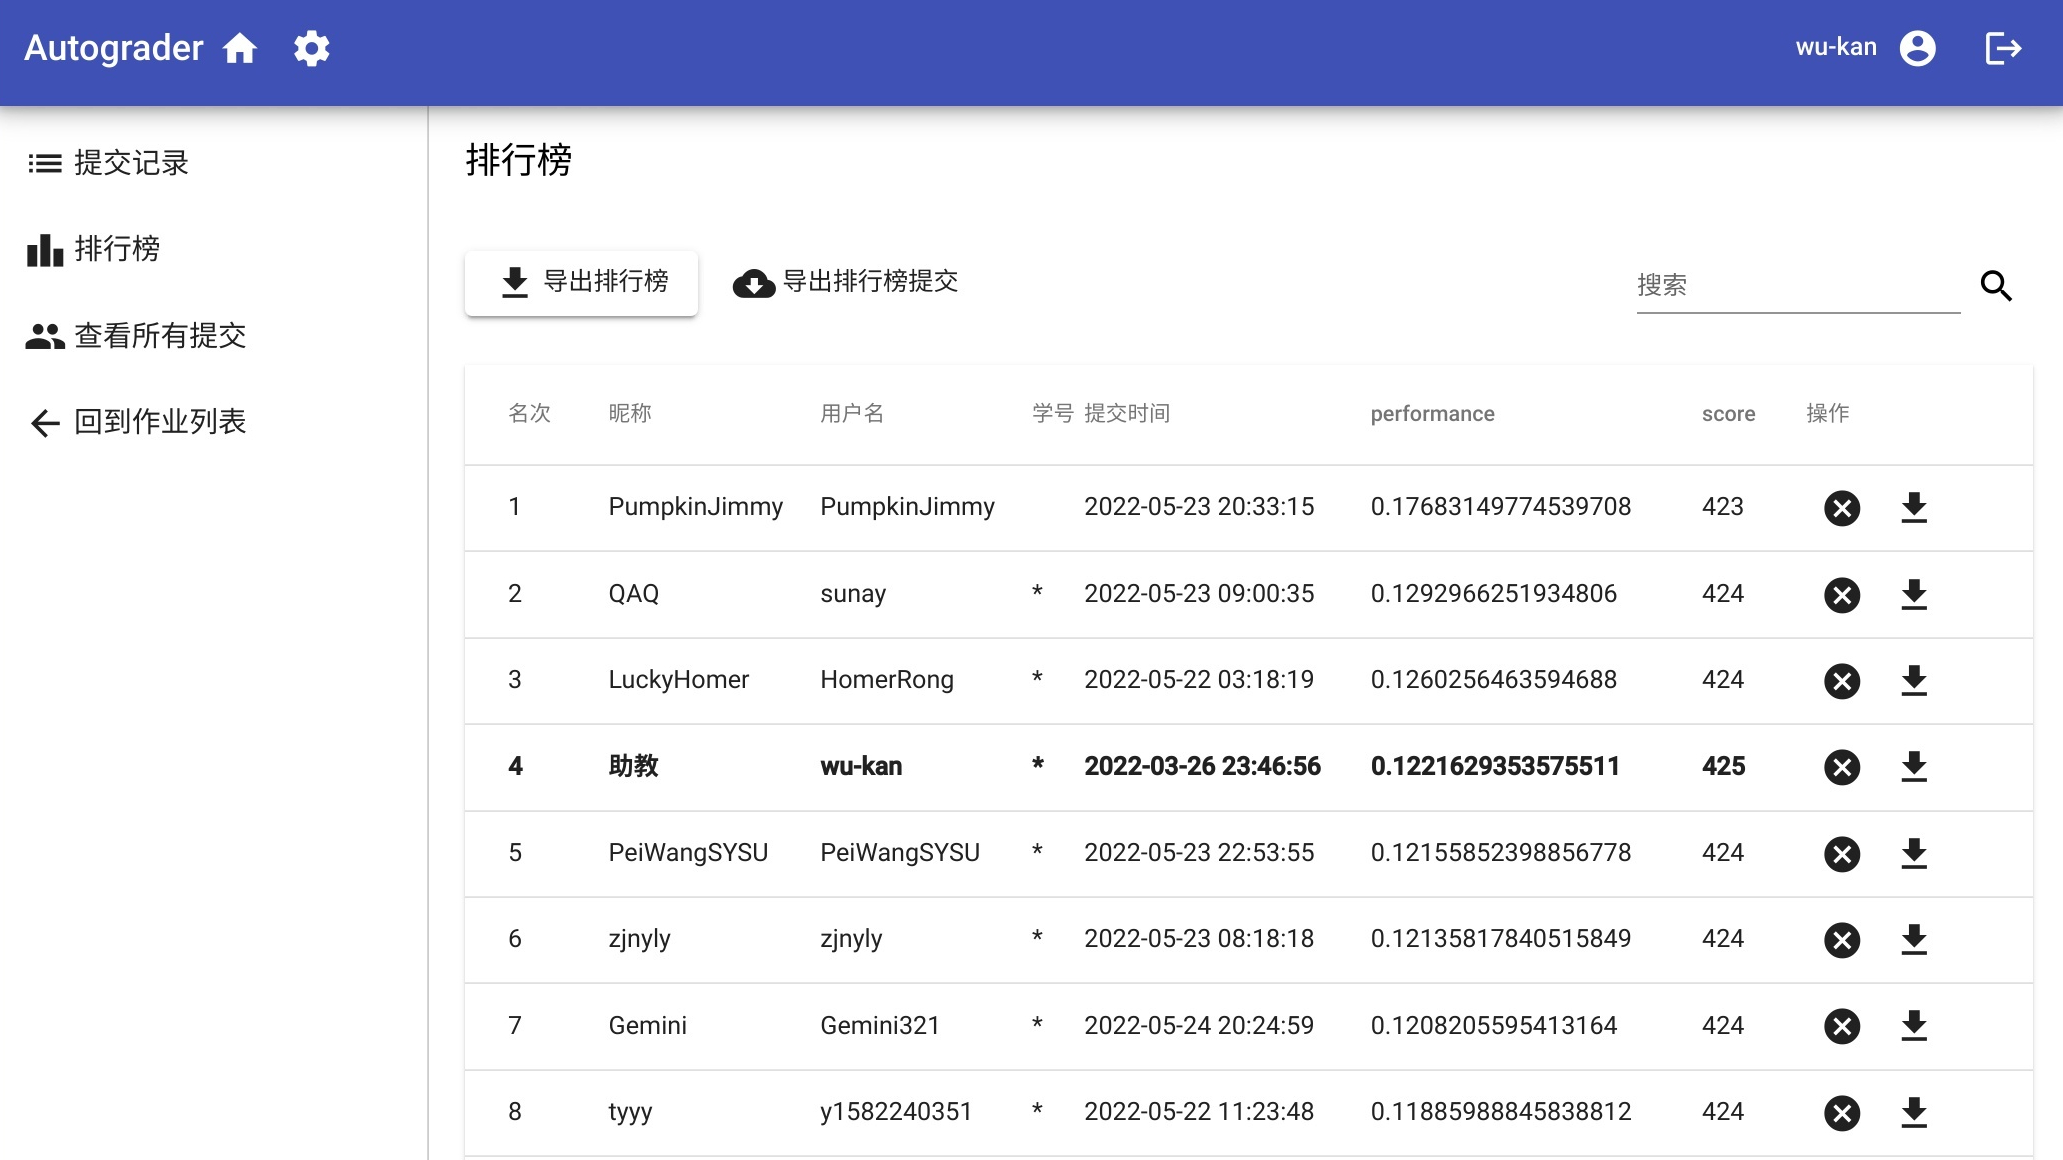
\includegraphics[width=0.9\textwidth]{assets/image/rank.jpg}
    \cnenfigcaption{在线评测与性能排名}{Caption}
    \label{rank}
\end{figure}

\textbf{完善开发环境,降低完成门槛}:我们认为,实验设计与难度不是证明教师和助教能力的舞台,而应该引导学生进行难度适宜的开发实践。考虑到课时的限制,编译实验在保证上述教学效果的同时整体工作量不宜过大,否则极易导致相当比例的学生无法正常跟上教学进度。为此,我们的实验设计借助LLVM库精简开发流程,定位于三千行左右实现一款相对完整的编译器,将目标代码生成设为可选以更凸显关键编译环节。同时,为方便学生上手,每个实验我们都提供了一定的模板代码以及完整的编译脚本,使得学生可以通过动手尝试快速进入实验状态。需要强调的是,所提供的模板代码通常不超过100行,从而方便学生对后续代码实现建立更为清晰的认知。此外,我们提供了完整的性能测评机制和排名(见图-\ref{rank}),以及详尽的测试用例,便于学生第一时间得到反馈,以用例促进实验开展。
%每个实验的模板都不超过一百行代码;完善的开发环境、ci测试、在线评测与排名(附图)

\textbf{重在基础、鼓励探索}:鉴于本科核心课程教育的基础性定位,本实验设计亦定位于编译经典知识的掌握,和通用编译技术的熟悉,而不刻意追求章节-\ref{sec_situation} 所述的 TVM 等前沿性内容。但考虑到部分学有余力学生的实际需要,我们充分鼓励在每个阶段性实验进行自由拓展和探索,并提供若干挑战问题和扩展建议,例如脱离 \texttt{bison} 自主实现文法解析、基于 AST 实现代码重构工具。同时,代码优化实验也不施加过多约束,鼓励学生考虑更灵活的优化方法,并与 {\tt clang -O3} 进行性能比对。机器代码生成同样作为可选实验,供学有余力学生完成,构建更为完整的编译器。
%聚焦编译经典技术,不刻意追求前沿(例如MLIR、TVM等);但,提供扩展建议,支持在完成基础实现之外自由探索。

\textbf{面向于编译、不止于编译}: 作为实际中软硬件衔接的关键,编译课程在计算机基础教学中也承担着贯穿程序设计、数据结构、组成原理和操作系统等多门课程的作用。因而,实验设计在满足编译教学需要的同时,也应促进学生对基础课程的融会贯通。对此,我们鼓励学生通过对所用精简 C 语言的编译构建,深入理解程序源代码到执行代码的流程,并添加所需语法实现“用自己开发的编译器编译自己的操作系统,并运行在自己设计的处理器上”的目标。此外,借助开源编译库的使用和二次开发,学生能够更好的完成从知识学习到能力提升的转换,提高问题分析求解和构建复杂工程的能力。
%从知识传授到能力培养的转换
%提升学生的工程技术创新能力
%对领域复杂问题进行分析、设计和实现的能力
%经历复杂系统的设计
%数据结构、离散数学、操作系统、组成原理、程序设计等
%提高学生通用问题求解能力和解决复杂工程问题的能力

%理解类C编程语言设计细节,通过实验理解源代码到执行代码的流程;可与组成原理、操作系统等基础性课程贯通;问题驱动,例如 json 处理性能带来的讨论

\section{具体实验方案}

围绕上述理念,我们基于Clang/LLVM自顶向下地设计了编译器构造实验框架,并使用木兰宽松许可证(第2版)\footnote{\url{https://github.com/arcsysu/SYsU-lang/blob/latest/LICENSE}} 开源于知名代码托管网站 GitHub。自项目开始的半年来已获得上百个星标,见图-\ref{github}。

\begin{figure}
    \centering
    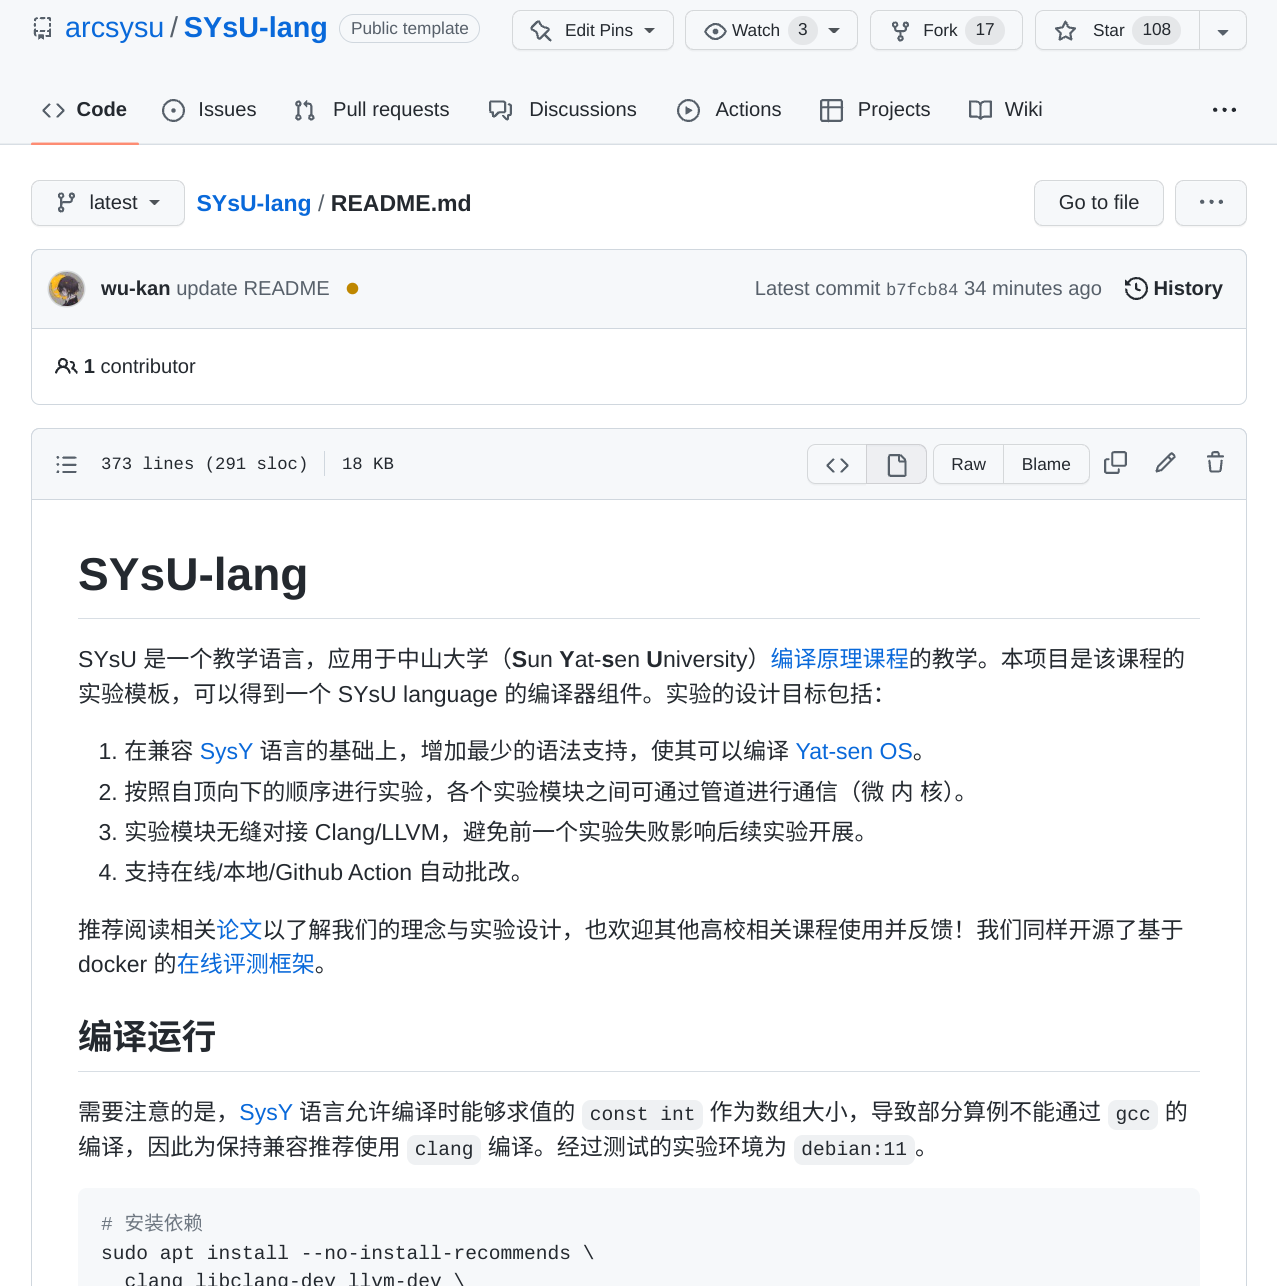
\includegraphics[width=0.9\textwidth]{{assets/image/github}}
    \cnenfigcaption{实验框架开源于 GitHub 平台}{Caption}
    \label{github}
\end{figure}

与其他高校相比,本实验特色之一是将完整编译器拆分为多个模块(如图-\ref{projs_overview} 所示),其中核心的词法分析、语法分析(语义分析)、中间代码生成、中间代码优化四个过程被设定为基础性必做实验;当学生完成从源代码转换到中间代码的完整流程后,即可认为已经完成一个完整的编译器构建。实验框架中包含了预处理器模块与生成汇编代码的后端模块,但并不强制要求学生必须完成,而是作为挑战项目供有兴趣、学有余力学生完成基本实验外自行实现并替换。除实现编译器的其他模块,完成必做实验本身也可以带来很多有趣的现实问题与挑战,将在下文中予以详细介绍。
%目标代码生成和链接部分作为可选实验,供学有余力学生完成。

\begin{figure}
    \centering
    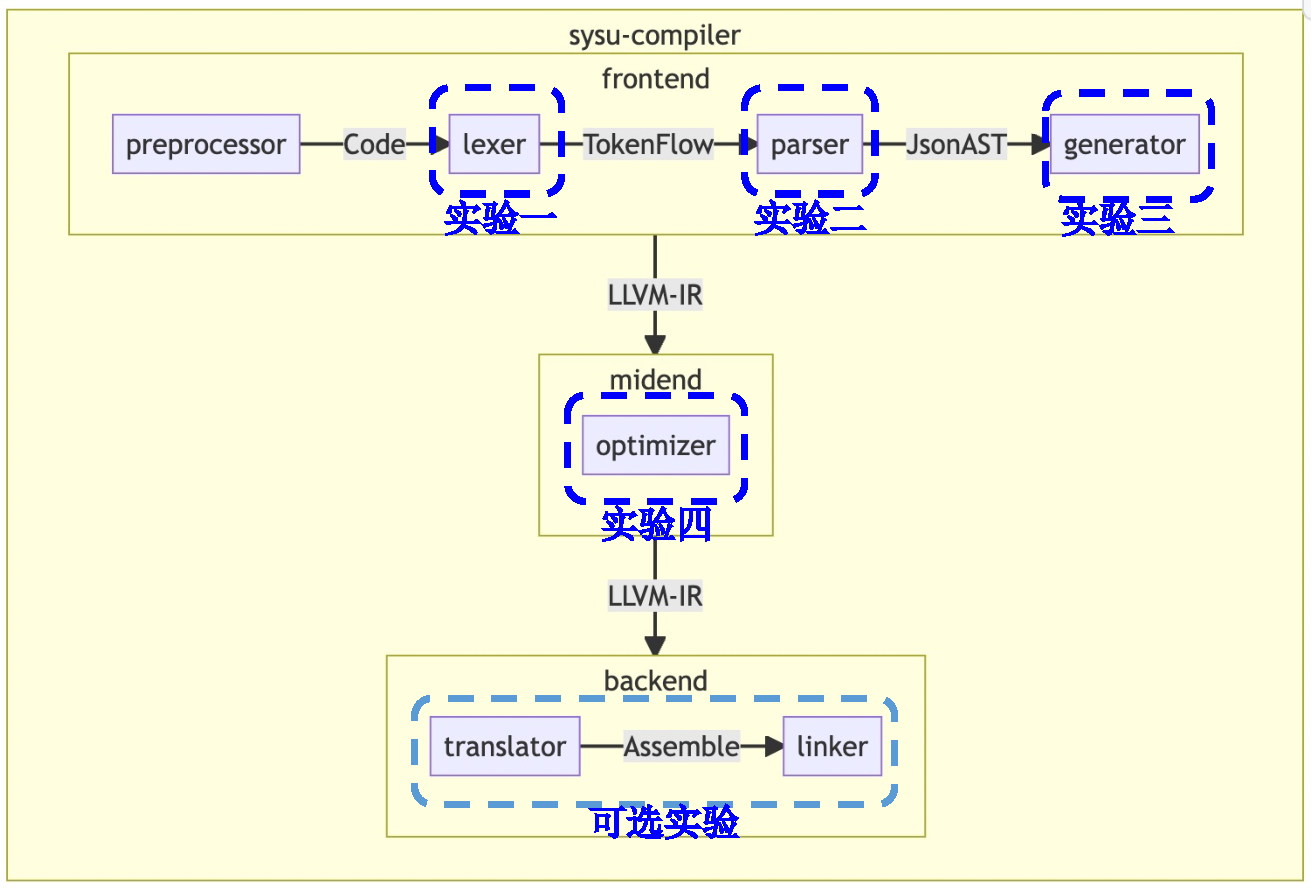
\includegraphics[width=0.9\textwidth]{{assets/image/projs_overview}.pdf}
    \cnenfigcaption{实验总体安排}{Caption}
    \label{projs_overview}
\end{figure}

\subsection{实验一:词法分析器}

作为第一个实验,词法分析实验设计上不宜难度过高,否则容易让学生产生畏难、抵触的情绪。作为简化,实验提供了一个约 90 行、基于 \texttt{flex} 的模板,学生需要在此基础上扩充其中的词法规则,实现完整的词法分析器,对输入的源代码进行分词、标注词性以及在源代码中的相对位置,完整实现代码量约为 250 行。实验同时提供了基于 \texttt{python} 编写的检验脚本,可以将学生的输出与Clang标准词法输出(\texttt{clang -cc1 -dump-tokens 2>\&1})进行比较,通过约 400 个算例的检查即视为通过。学生可以通过本地执行检验脚本或是 GitHub Action 完成结果检查,耗时约 20秒 ~ 3 分钟,不会影响实验正常进展。

\subsection{实验二:语法分析器}

自实验二开始,难度阶梯上升,学生将在实践中锻炼自己工程实现能力,并一窥 LLVM 的真面目。实验二工作量上设计为约1000行代码
%,耗时 24 小时 ~ 72 小时
。

实验二任务为完成一个语法分析器,接受来自实验一或者 \texttt{clang -cc1 -dump-tokens 2>\&1} 的输入,输出 JSON 格式的语法树;检测脚本将把Clang标准AST(\texttt{clang -cc1 -ast-dump=json})与学生的输出进行比较,同时遍历两棵语法树,检查每一个节点是否正确。

需要说明的是,考虑到实验二本身的难度跃升,我们对复杂的语法/语义分析进行了简化,并不要求学生手写递归下降法或移进归约来完成这一过程,而是使用成熟的\texttt{bison} 自动解析工具来降低实验难度。基于形式自动机理论实现语法分析的知识已经足够成熟,而掌握 \texttt{bison} 工具的使用,对快速实现一门语言的需求更加具有现实意义。另外,实验二的 SYsU 文法是 SysY 文法的一个稍微扩展,文法的 EBNF 定义\cite{sysy} 完整,资料丰富,文法本身十分精简,在教师和助教的帮助下,学生预期能够以 1000 行左右的代码量完成实验。

实验二要求输出为 JSON 格式的语法树,并提供了基于 \texttt{bison} + \texttt{llvm::json} 的约100行代码模板。这样的设计至少有以下三点好处:1)便于使用 \texttt{python} 脚本和 \texttt{clang} 导出的语法树对比,自动批改;2)JSON 格式非常容易理解与上手,不需要像 LLVM 官方教程\cite{llvm_manual1}一样定义很多节点;3)可以让学生提前上手 LLVM 开发库的使用,平滑下一个实验的难度。
此外,实验模板也尽量避免使用 \texttt{bison} 提供的一些机制,而是使用了一个自行构造的栈用于语法分析的中转,让学生理解``移进-规约''的过程。例如,遇到悬垂 else 等可能会出现二义性的情况时,\texttt{bison} 使用的 LALR(1) 文法会向前多检测一次 token,学生如果不注意便会从栈中取出错误的节点。

\begin{figure}
    \centering
    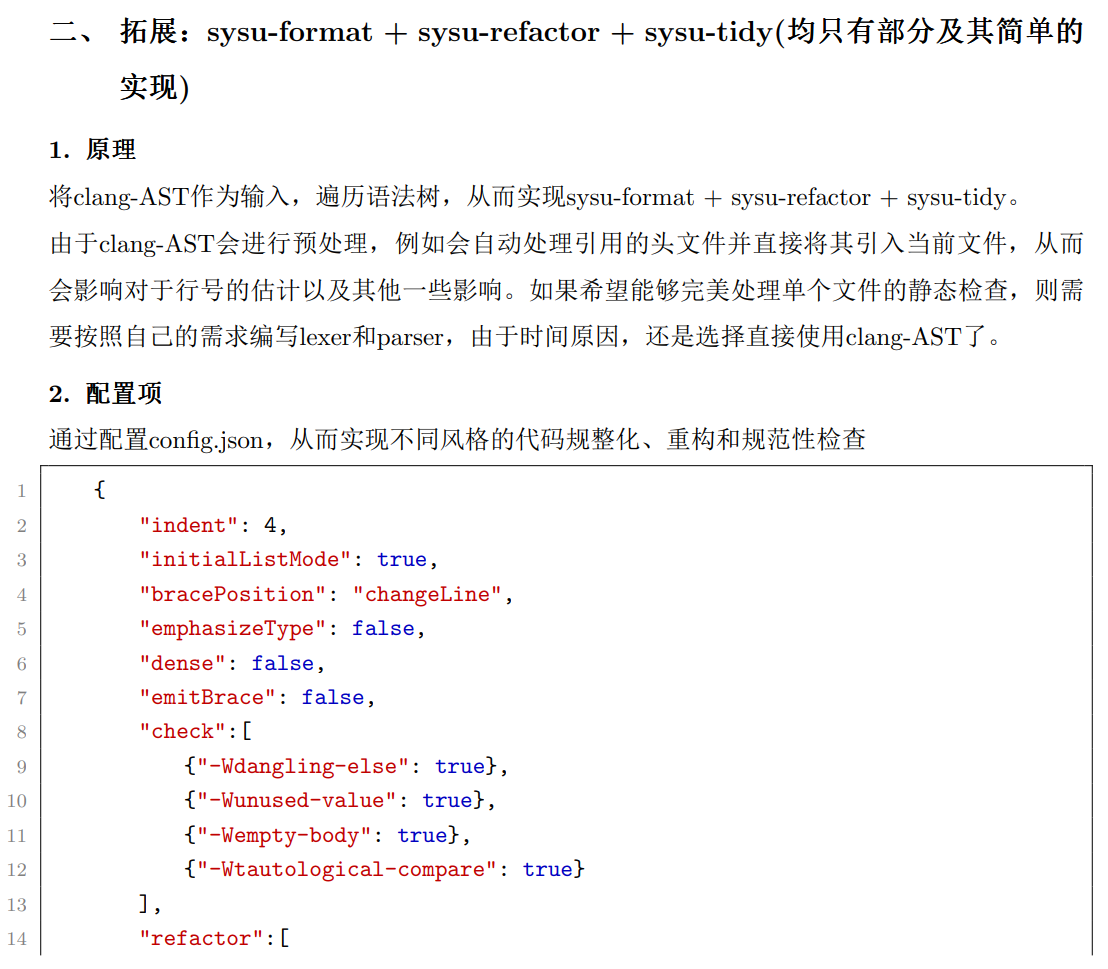
\includegraphics[width=0.9\textwidth]{assets/image/report1}
    \cnenfigcaption{学生基于实验二实现的小工具}{Caption}
    \label{report1}
\end{figure}

经过实验二,学生得到了精简 C 语言的语法树,此时也可以引入关于 \texttt{clang-format}、\texttt{clang-tidy}、\texttt{clang-refactor}、\texttt{clangd} 等基于 \texttt{clang} 的现代化开发工具介绍。如图-\ref{report1},学生在体验现代化编译工具带来的便利后,甚至可以额外实现一套简单的代码规范检查、规整化、重构工具。

\subsection{实验三:IR 生成器}

难度在实验三达到峰值,学生将完全进入LLVM开发范畴。本实验要求学生完成一个 IR生成器,接受来自实验二或者 \texttt{clang -cc1 -ast-dump=json} 的输入,输出 LLVM IR;检测脚本会通过 \texttt{clang -cc1 -O3 -S -emit-llvm} 得到用于对比的 LLVM IR;两份 IR 将同时通过 \texttt{llc -O0} 编译成二进制可执行文件,随后比较该文件执行时的输出与返回值。完成实验三预期需要 1500 行代码。
%,耗时 36 小时 ~ 108 小时。

实验三带给学生的意义,除了完成一个完整的编译器外,还可以自然地启发学生编译器和计算机硬件是怎样认识我们编写的代码的,从而自然地领悟一些优秀的编程习惯。例如 C 语言中的短路运算,看起来有时可以规避掉一些不必要的计算,但是实验中将其转换为中间代码表示时却需要一些复杂的跳转指令,很多时候并不如直接使用位运算。

在学生完成实验三时,一些特殊的算例并不能在评测机的时限内运行完成,此处即可引出实验四的 IR 优化实验。此外还会遇到一个非常有意义的问题:在处理一个语法树深度达到数十万的大算例时,模板中使用的 \texttt{llvm::json::parse} 性能难以满足要求,在评测机上需要运行十五分钟才能将其完全解析,而作为对照,\texttt{python} 中的 \texttt{json.loads} 仅需要八秒。实验中同样允许超时跳过这一算例,但是学生也同样被鼓励使用编译原理课程上学到的知识,实现一个高性能的 JSON 处理库,并与一些高性能的实现做对比。

\subsection{实验四:IR 优化器}
有别与前三个实验,实验四更具开放性,没有预期完成时间与代码行数。基本要求是,完成一个 IR 优化器,接受来自实验三或 \texttt{clang -cc1 -O0 -S -emit-llvm} 的 LLVM IR,输出优化后的 LLVM IR。学生在本实验中需要编写 LLVM Pass,重点面向实验三中的三类超时情况进行优化,即:死代码消除、公共子表达式提取、常量除法转换。

值得一提的是,实验四关注的 Pass/PassManager 是 LLVM 里最重要的核心组件之一,自 LLVM 诞生以来已经有数十年历史。由于原有的 PM 编译效率低且错失很多优化机会,2014 年开始 LLVM 团队对其开始重构。和其他高校的实验相比,我们的实验设计上有后发优势,在实验环境中使用的 LLVM-11 虽然默认使用的仍然是旧 PM,但已经包含新 PM,学生也被鼓励去写新规格的 LLVM Pass。

学生在实验四中的得分由在线评测中与\texttt{clang -cc1 -O3 -S -emit-llvm} 运行时间的比值决定。这样的评分方式下,学生很难获得满分,因此此处鼓励学生完成几个实验中的挑战选项以获取额外的加分。

\section{初步评估}
基于上述设计,我们在2022年春季学期于中山大学计算机学院开展了实验教学。课程为《编译器构造实验》,与《编译原理》同为必修课程,面向计算机科学与技术专业大三学生,跨度为完整学期,共20周1学分36学时。实验课堂规模为60人,1名任课教师,3名助教。每项实验要求学生提交完成代码和简短实验报告,报告内容,特别是心得部分,不做强制性要求,不计入评分,以获得最真实的反馈。以下为此次教学的初步数据统计和反馈收集。

\subsection{教学反馈}
在实际的教学过程中,我们根据难度和工作量对各实验预留了不同的完成时间(见表-\ref{projs})。
%这四个实验的难度总体是一个先递增后减的过程,其中在实验三的中间代码生成难度达到最值。
学生完成的时间也由最开始词法分析的2 天到中间代码生成3周的过程,代码量相应由250行到1500 行的递增。

\begin{table}
    \centering
    \cnentablecaption{实验任务量及时间安排}{Caption}
    \label{projs}
    \footnotesize
    \tabcolsep 19pt %space between two columns. 用于调整列间距
    \begin{tabular*}{1.0\textwidth}{ccccc}
        \toprule
        实验 & 内容 & 代码量(行数/LOC) & 用时(小时/h) & 预留时间(天/d) \\\hline
        一 & 词法分析器/lexer & 250 & 2 - 6 & 14\\
        二 & 语法分析器/parser & 1000 & 24 - 72 & 30\\
        三 & IR生成器/generator & 1500 & 36 - 108 & 30\\
        四 & IR优化器/optimizer & 开放性实验,推荐值为 500 & 24 - 150 & 30\\
        \bottomrule
    \end{tabular*}
\end{table}

%\begin{figure}
%\centering
%\includegraphics[width=0.65\textwidth]{{assets/image/proj_hrs}.pdf}
%\cnenfigcaption{实验统计完成用时}{Caption}
%\label{proj_hrs}
%\end{figure}

%具体而言,实验一的耗时主要体现在对实验环境的熟悉(如 Linux 环境,命令行的使用等),基于 \texttt{flex} 识别正则表达式从而完成词法分析大大减低了实验难度,代码量总体 200 行以内。

实验一基于\texttt{flex}识别正则表达式从而完成词法分析大大减低了实验难度,代码量总体约 200 行,耗时约 2 到 6 小时。经学生反馈,其中主要的难点是使用正则表达式描述包含转义字符的 C 语言字符串。此外,超过半数的学生并没有熟练使用命令行与 Unix/Linux 工具链的经验;学生完成实验一期间的提问主要集中在实验环境部署、环境变量、头文件/库文件/可执行文件缺失上,非常适合以此作为切入点,进行一次 Linux 使用与常用指令的教学。

实验二相比实验一,在难度上有明显提升。在实验早期,大部分学生并不完全理解需要做的工作;而少部分能力强的学生也质疑是否能够完成。在课程教学中,我们的解决方法是:由教师制作详细的实验原理指导\footnote{\url{https://xianweiz.github.io/teach/dcs290/slides-22/lab_7.pdf}},同时建立在线问答平台\footnote{\url{https://github.com/arcsysu/SYsU-lang/discussions}},由助教与具有解决经验的学生共同答疑,鼓励学生就遇到的问题多多提问。最终,大三年级学生中约 90\% 可以在规定期限内顺利完成,其余学生在适当延期和额外指导下也能陆续提交。如图-\ref{tucao} 和图-\ref{report2} 所示,学生在对语法树操作过程中备感挑战的同时也在完成之际收获了极大成就感。

\begin{figure}
    \centering
    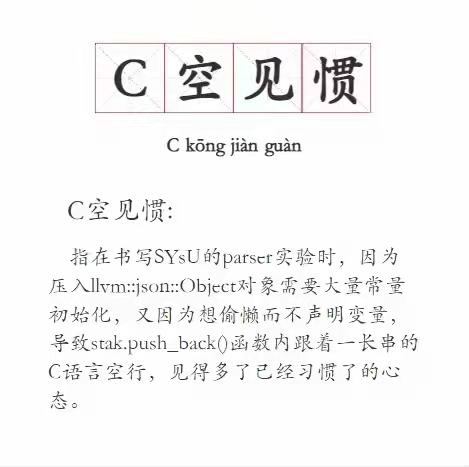
\includegraphics[width=0.3\textwidth]{assets/image/tucao.jpg}
    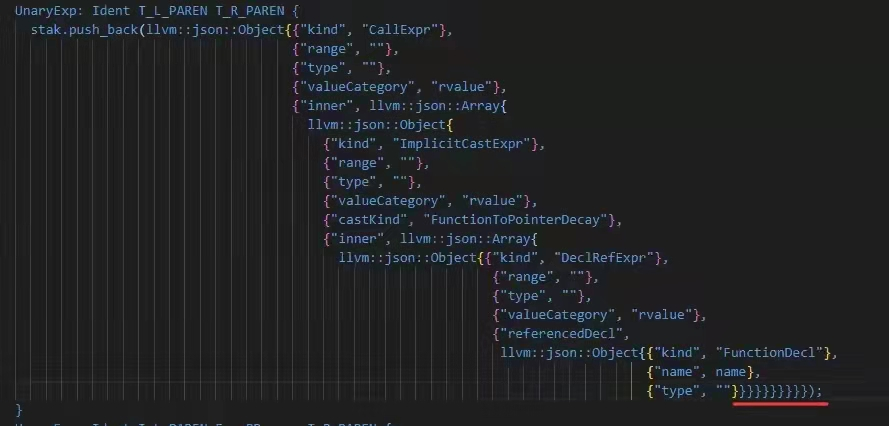
\includegraphics[width=0.6\textwidth]{assets/image/tucao1.jpg}
    \cnenfigcaption{学生完成实验二之余制作的表情包,苦中作乐}{Caption}
    \label{tucao}
\end{figure}

\begin{figure}
    \centering
    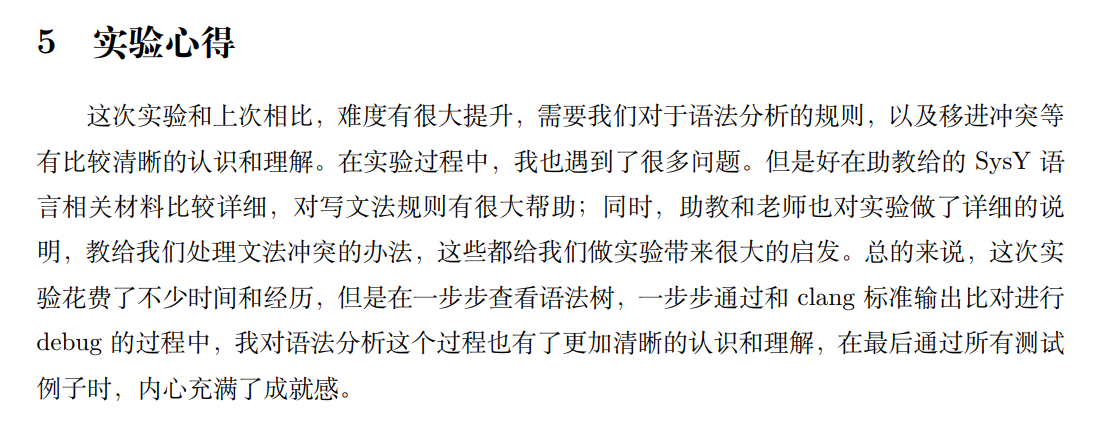
\includegraphics[width=0.9\textwidth]{assets/image/report2}
    \cnenfigcaption{学生实验二心得}{Caption}
    \label{report2}
\end{figure}

实验三是本编译实验的核心和精髓,同时也是四个实验中挑战最大的一个。中间代码的生成标志着编译器前端工作结束、正式进入中端范畴,生成 LLVM IR 的必备知识包含LLVM/IR 本身\cite{llvm_manual}的表示规则和生成 LLVM/IR 的 LLVM/IR 库使用方法,二者的理解和掌握需要花费不少时间。实际编写程序也需要考虑众多问题:比如语法树递归遍历,多维数组处理,if/else控制分支语句处理,短路运算求值过程等,非常考验学生的算法和数据结构能力。此外,学生在实验三遇到的另一个难题是:LLVM库本身的更新与重构过于频繁,很多时候文档并没有跟上;优质的中文资料更是偏少。在实验中我们由助教与学生同时完成了实验三,并编写中文指导文档,标注一些实验中可能会使用到的LLVM API与使用方法。%从目前学生完成普遍情况来看,实验三的代码量在 1500 行左右。

%\textcolor{red}{所幸经过实验二的风波,学生在面对实验三时不再首先质疑实验是否可以完成。但是学生在实验三遇到的一个难题是:LLVM 库本身的更新与重构过于频繁,很多时候文档并没有跟上;优质的中文资料更是偏少。在实验中我们由助教与学生同时完成了实验三,并编写中文指导文档,标注一些实验中可能会使用到的 LLVM API 与使用方法。}

实验四是开放性实验,其难度完全由学生自行把控,追求性能优化的同时将伴随编程工作量的上升。但是一些常见的优化技巧,比如死代码消除等资料较为丰富,预计的代码量在500 行左右。截至论文投稿日(2022年5月31日),实验四发布时长不超过一周,但已有学生将编译器的性能从开始的12\%(与 \texttt{clang -O0} 相当)提高到24\%,加速比超过 100\%,总体来说非常值得期待。

拓展性实验方面,在完成实验基本任务之外,不少学生积极进行探索,尝试完成一些挑战性工作。图-\ref{report1} 展示了学生在实验二中利用JSON进行的代码格式规整化和规范检查的工具开发。尽管实验四尚在进行中,部分学生已经对后继机器代码生成进行了思考。

\subsection{主要挑战及问题}
根据学生的反馈,实验目前的挑战和问题主要体现在以下方面:

\begin{enumerate}
    \item SYsU文法和Clang语法树:在实验二开展过程中,SYsU文法实际上是在SysY文法基础上稍微进行了扩展,所以文法本身并不会特别复杂。在根据文法实现语法分析的过程,实验中允许学生使用\texttt{bison} 等语法分析工具,没有强制学生手写递归下降或规约推导方法来实现,减少了语法分析的实现复杂性。实验二要求学生生成一棵和 Clang 生成对比的 JSON 语法树,而 Clang 语法树具有明确规律的生成规则和语义,其具体的结点生成规则。如图-\ref{report2} 学生实验报告写道,语法树的规则可以通过自己手动编译测试样例生成 JSON语法树,进行观察从而掌握。当然,在未来的编译原理实验教学中,我们将给出具体明确的Clang的JSON 语法树生成规则,以进一步降低实验的难度。
    \item 教程和帮助文档:由于 LLVM 的文档 \cite{llvm_newpass} 很多时候赶不上其开发速度,一些 API 的功能描述略少,导致学生在着手开展实验时存在短期的不适应。但是,实验中用到的很多 LLVM IR 部分的API 并不会特别复杂,完成实验需要使用的API数量有限,加上老师和助教的引导,没有成为学生完成实验的绊脚石。然而,如图-\ref{complain} 所示,部分学生还是在实验过程中不得不对代码进行多次重构。为尽量避免此类问题频繁发生,我们后续将对本实验中使用到的 LLVM 相关API编写详细实用说明文档,提供给将来开展的编译原理实验教学。与此同时,我们也计划邀请本届学生参与到后续的课程建设和改进中,在代码和文档方面进行持续性改进。
\end{enumerate}

\begin{figure}
    \centering
    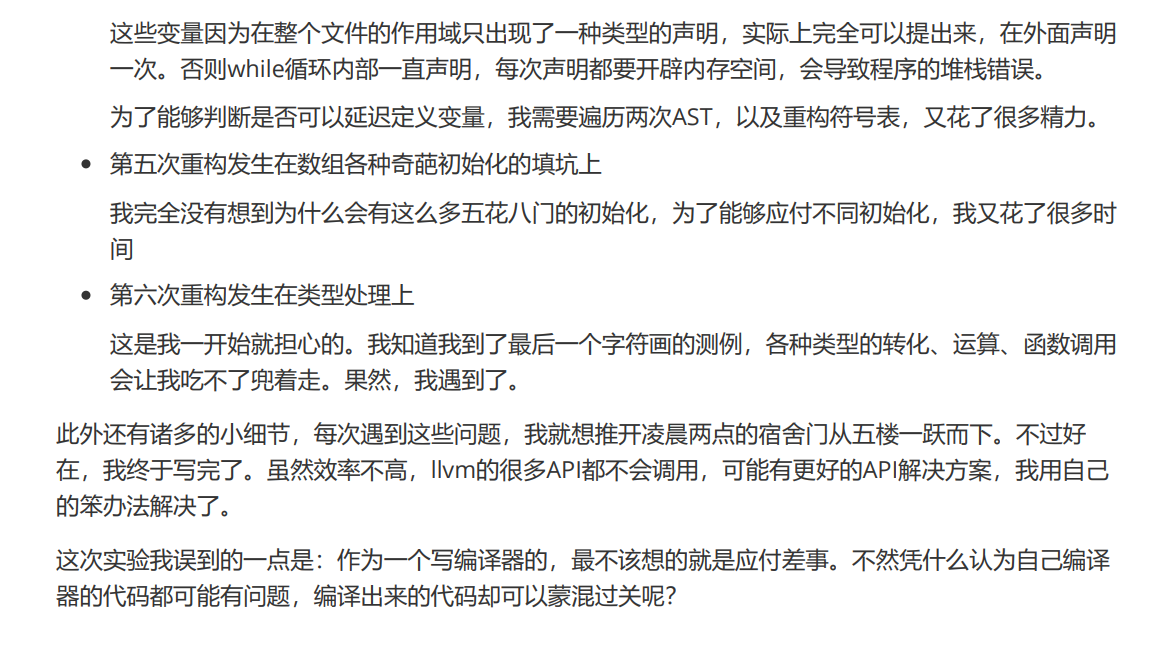
\includegraphics[width=0.9\textwidth]{assets/image/report}
    \cnenfigcaption{学生在实验中会面临需要多次重构的情况}{Caption}
    \label{complain}
\end{figure}

这些挑战于我们是实验的改进方向,于学生是潜在的经验财富。通过实验历练,学生对 CMake、Linux 命令等系统开发工具和技术的掌握,无论将来是否从事编译领域的研究或工作,都将裨益其计算机职业生涯。

\section{总结与展望}
为更好的满足现代计算机专业领域所要求的人才培养需求,在综合分析和借鉴国内外相关课程设置的基础上,我们面向中山大学计算机专业教学实际,设计了基于Clang/LLVM的模块化和解耦化编译实验,在聚焦编译核心技术学习和掌握的同时,侧重培养学生的系统观、全局观。初步的教学结果表明,所设计的编译教学实验有效提高了实践性和实用性。

后续我们将对实验进行持续性完善和提升,一些可能的后续计划如下:参照 \texttt{flang} 等开源编译器实现,探索将 MLIR 等 LLVM 前沿组件引入课程实验的可能性;完善可选的后端(RISC-V,ARM,X86)与 JIT 模块实验设计,供有兴趣、有能力的学生挑战;使用 SYsU 文法实现各个实验模块,实现编译器的自举;将 SYsU-lang 加入教育平台超算习堂的在线实训\footnote{\url{https://easyhpc.net/lab}},进一步降低实验门槛、扩大受众范围;与中山大学操作系统、组成原理实验课程进行软硬协同设计,使用相同的实验环境,以最少的代码量达成“用自己开发的编译器\footnote{\url{https://github.com/arcsysu/SYsU-lang}}编译自己的操作系统\footnote{\url{https://github.com/YatSenOS/YatSenOS-Tutorial-Volume-1}},并运行在自己设计的处理器\footnote{\url{https://yatcpu.sysu.tech}}上”这一目标,培养出时代真正需要的、具有软硬系统大局观的学生。

%%%%%%%%%%%%%%%%%%%%%%%%%%%%%%%%%%%%%%%%%%%%%%%%%%%%%%%
%%% 致谢
%%% 非必选
%%%%%%%%%%%%%%%%%%%%%%%%%%%%%%%%%%%%%%%%%%%%%%%%%%%%%%%
%\Acknowledgements{致谢.}

%%%%%%%%%%%%%%%%%%%%%%%%%%%%%%%%%%%%%%%%%%%%%%%%%%%%%%%
%%% 补充材料说明
%%% 非必选
%%%%%%%%%%%%%%%%%%%%%%%%%%%%%%%%%%%%%%%%%%%%%%%%%%%%%%%
%\Supplements{补充材料.}

%%%%%%%%%%%%%%%%%%%%%%%%%%%%%%%%%%%%%%%%%%%%%%%%%%%%%%%
%%% 参考文献, {}为引用的标签, 数字/字母均可
%%% 文中上标引用: \upcite{1,2}
%%% 文中正常引用: \cite{1,2}
%%%%%%%%%%%%%%%%%%%%%%%%%%%%%%%%%%%%%%%%%%%%%%%%%%%%%%%
\begin{thebibliography}{99}
    \bibitem{moe21_101}高教创时代, 教育部全面实施教育数字化战略行动 构建中国特色高等教育数字化新体系, \url{https://m.eol.cn/toutiao/202203/t20220328_2217408.shtml}
    %\textcolor{gray}{教育部101计划:通过包括编译在内的12门核心课程的深度改革和建设,“探索计算机领域人才培养的新理念、新内容、新方法,引领带动高校人才培养质量的整体提升”,“实现教育链、产业链和创新链深度融合”。}

    \bibitem{moe22_file}教育部,教育部高等教育司2022年工作要点, \url{http://www.moe.gov.cn/s78/A08/tongzhi/202203/W020220310547779354544.pdf}
    %\textcolor{gray}{加强紧缺人才培养、深入实施“六卓越一拔尖”计划 2.0}
    \bibitem{web_llvm} Colfaxresearch, A Performance-Based Comparison of C/C++ Compilers, \url{https://colfaxresearch.com/compiler-comparison/}

    \bibitem{chris21_golden} Chris Lattner, ASPLOS Keynote: The Golden Age of Compiler Design in an Era of HW/SW Co-design, \url{https://tenstorrent.com/research/asplos-keynote-the-golden-age-of-compiler-design-in-an-era-of-hw-sw-co-design-by-dr-chris-lattner/}

    \bibitem{nv_c} NVIDIA, CUDA LLVM Compiler, \url{https://developer.nvidia.com/cuda-llvm-compiler}
    \bibitem{olcf19_c} Philip C. Roth, Experiences with the Heterogeneouscompute Interface for Portability (HIP) on
    OLCF Summit, \url{https://www.olcf.ornl.gov/wp-content/uploads/2019/10/Roth-HIP-on-Summit-20191009.pdf}
    \bibitem{tpu_c} Coral, Edge TPU Compiler, \url{https://coral.ai/docs/edgetpu/compiler}
    \bibitem{intel21_c} Intel, Intel C/C++ compilers complete adoption of LLVM, \url{https://www.intel.com/content/www/us/en/developer/articles/technical/adoption-of-llvm-complete-icx.html}
    \bibitem{ibm20_c} IBM, IBM C/C++ and Fortran compilers to adopt LLVM open source infrastructure, \url{https://developer.ibm.com/blogs/c-and-fortran-adopt-llvm-open-source}

    \bibitem{mlir} LLVM, MLIR: Multi-Level IR Compiler Framework, \url{https://mlir.llvm.org/}

    \bibitem{tvm21_c} Apache, Apache TVM: An End to End Machine Learning Compiler Framework for CPUs, GPUs and accelerators, \url{https://tvm.apache.org/}

    \bibitem{zhong18_blockchain} Robin Zhong, LLVM x Blockchain: A New Ecosystem of Decentralized Applications, \url{https://llvm.org/devmtg/2018-04/slides/Zhong-LLVM\%20x\%20Blockchain.pdf}

    \bibitem{ndss18_zeus} Sukrit Kalra and Seep Goel, et al. ZEUS: Analyzing Safety of Smart Contracts, In Network and Distributed Systems Security (NDSS) Symposium, San Diego, CA, USA, 2018.
    \bibitem{ms20_qir} Microsoft, Introducing Quantum Intermediate Representation (QIR), \url{https://devblogs.microsoft.com/qsharp/introducing-quantum-intermediate-representation-qir/}
    \bibitem{arxiv22_qc} Pradnya Khalate and Xin-Chuan Wu, et al. An LLVM-based C++ Compiler Toolchain for Variational Hybrid Quantum-Classical Algorithms and Quantum Accelerators, \url{https://arxiv.org/pdf/2202.11142.pdf}

    \bibitem{huawei_c}华为, 毕昇编译器介绍, \url{https://support.huaweicloud.com/ug-bisheng-kunpengdevps/kunpengbisheng\_06\_0001.html}
    \bibitem{baidu_c}百度, 源于产业实践的开源深度学习平台, \url{https://www.paddlepaddle.org.cn/}
    \bibitem{llvm_manual1} LLVM Compile Infrastructure, LLVM Language Reference Manual,
    \url{https://releases.llvm.org/11.0.1/docs/tutorial/MyFirstLanguageFrontend/LangImpl02.html}
    \bibitem{llvm_manual} LLVM Tutorial, Kaleidoscope: Implementing a Parser and AST, \url{https://releases.llvm.org/11.0.1/docs/LangRef.html}
    \bibitem{llvm_newpass} LLVM Compile Infrastructure, Using the New Pass Manager, \url{https://llvm.org/docs/NewPassManager.html}
    \bibitem{stanford_cs143} Stanford University, CS143: Compilers, \url{https://web.stanford.edu/class/cs143/}
    \bibitem{cornell_cs1620} Cornell University, CS 6120: Advanced Compilers, \url{https://www.cs.cornell.edu/courses/cs6120/2019fa/project/}
    \bibitem{thu21_compiler} 清华大学, MiniDecaf 编译实验, \url{https://github.com/decaf-lang/minidecaf-tutorial}

    \bibitem{pku20_compiler} 北京大学, PKU compiler course online documentation, \url{https://github.com/pku-minic/online-doc}
    \bibitem{buaa19_compiler} 北京航空航天大学, miniSysY 编译实验, \url{https://github.com/buaa-se-compiling/miniSysY-tutorial}
    \bibitem{sysy}
    全国大学生计算机系统能力大赛——编译系统设计赛,SysY语言定义,\url{https://gitlab.eduxiji.net/nscscc/compiler2021/-/blob/master/SysY\%E8\%AF\%AD\%E8\%A8\%80\%E5\%AE\%9A\%E4\%B9\%89.pdf}
    %\bibitem{author} 张三, 李四, Author C, et al. Reference title. In: Proceedings of Conference, Place, Year. Number or pages

\end{thebibliography}

%%%%%%%%%%%%%%%%%%%%%%%%%%%%%%%%%%%%%%%%%%%%%%%%%%%%%%%
%%% 附录章节, 自动从A编号, 以\section开始一节
%%% 非必选
%%%%%%%%%%%%%%%%%%%%%%%%%%%%%%%%%%%%%%%%%%%%%%%%%%%%%%%
%\begin{appendix}
%\section{附录}
%附录从这里开始.
%\begin{figure}[H]
%\centering
%%\includegraphics{fig1.eps}
%\cnenfigcaption{附录里的图}{Caption}
%\label{fig1}
%\end{figure}
%\end{appendix}


%%%%%%%%%%%%%%%%%%%%%%%%%%%%%%%%%%%%%%%%%%%%%%%%%%%%%%%
%%% 自动生成英文标题部分
%%%%%%%%%%%%%%%%%%%%%%%%%%%%%%%%%%%%%%%%%%%%%%%%%%%%%%%
%\makeentitle


%%%%%%%%%%%%%%%%%%%%%%%%%%%%%%%%%%%%%%%%%%%%%%%%%%%%%%%
%%% 主要作者英文简介, 数量不超过4个
%%% \authorcv[zp1.eps]{Ming XING}{was born in ...}
%%% [照片文件名]请提供清晰的一寸浅色背景照片, 宽高比为 25:35
%%% {姓名}与英文标题处一致
%%%%%%%%%%%%%%%%%%%%%%%%%%%%%%%%%%%%%%%%%%%%%%%%%%%%%%%
%\authorcv[]{Ming XING}{was born in ...}

%\authorcv[]{Ming XING}{was born in ...}

%\vspace*{6mm} % 调整照片行间距

%\authorcv[]{Ming XING}{was born in ...}

%\authorcv[]{Ming XING}{was born in ...}



%%%%%%%%%%%%%%%%%%%%%%%%%%%%%%%%%%%%%%%%%%%%%%%%%%%%%%%
%%% 补充材料, 以附件形式作网络在线, 不出现在印刷版中
%%% 不做加工和排版, 仅用于获得图片和表格编号
%%% 自动从I编号, 以\section开始一节
%%% 可以没有\section
%%%%%%%%%%%%%%%%%%%%%%%%%%%%%%%%%%%%%%%%%%%%%%%%%%%%%%%
%\begin{supplement}
%\section{supplement1}
%自动从I编号, 以section开始一节.
%\begin{figure}[H]
%\centering
%\includegraphics{fig1.eps}
%\cnenfigcaption{补充材料里的图}{Caption}
%\label{fig1}
%\end{figure}
%\end{supplement}

\end{document}


%%%%%%%%%%%%%%%%%%%%%%%%%%%%%%%%%%%%%%%%%%%%%%%%%%%%%%%
%%% 本模板使用的latex排版示例
%%%%%%%%%%%%%%%%%%%%%%%%%%%%%%%%%%%%%%%%%%%%%%%%%%%%%%%

%%% 章节
\section{}
\subsection{}
\subsubsection{}


%%% 普通列表
\begin{itemize}
    \item Aaa aaa.
    \item Bbb bbb.
    \item Ccc ccc.
\end{itemize}

%%% 自由编号列表
\begin{itemize}
    \itemindent 4em
    \item[(1)] Aaa aaa.
    \item[(2)] Bbb bbb.
    \item[(3)] Ccc ccc.
\end{itemize}

%%% 定义、定理、引理、推论等, 可用下列标签
%%% definition 定义
%%% theorem 定理
%%% lemma 引理
%%% corollary 推论
%%% axiom 公理
%%% propsition 命题
%%% example 例
%%% exercise 习题
%%% solution 解名
%%% notation 注
%%% assumption 假设
%%% remark 注释
%%% property 性质
%%% []中的名称可以省略, \label{引用名}可在正文中引用
\begin{definition}[定义名]\label{def1}
    定义内容.
\end{definition}



%%% 单图
%%% 可在文中使用图\ref{fig1}引用图编号
\begin{figure}[!t]
    \centering
    \includegraphics{fig1.eps}
    \cnenfigcaption{中文图题}{Caption}
    \label{fig1}
\end{figure}

%%% 并排图
%%% 可在文中使用图\ref{fig1}、图\ref{fig2}引用图编号
\begin{figure}[!t]
    \centering
    \begin{minipage}[c]{0.48\textwidth}
        \centering
        \includegraphics{fig1.eps}
    \end{minipage}
    \hspace{0.02\textwidth}
    \begin{minipage}[c]{0.48\textwidth}
        \centering
        \includegraphics{fig2.eps}
    \end{minipage}\\[3mm]
    \begin{minipage}[t]{0.48\textwidth}
        \centering
        \cnenfigcaption{中文图题1}{Caption1}
        \label{fig1}
    \end{minipage}
    \hspace{0.02\textwidth}
    \begin{minipage}[t]{0.48\textwidth}
        \centering
        \cnenfigcaption{中文图题2}{Caption2}
        \label{fig2}
    \end{minipage}
\end{figure}

%%% 并排子图
%%% 需要英文分图题 (a)...; (b)...
\begin{figure}[!t]
    \centering
    \begin{minipage}[c]{0.48\textwidth}
        \centering
        \includegraphics{subfig1.eps}
    \end{minipage}
    \hspace{0.02\textwidth}
    \begin{minipage}[c]{0.48\textwidth}
        \centering
        \includegraphics{subfig2.eps}
    \end{minipage}
    \cnenfigcaption{中文图题}{Caption}
    \label{fig1}
\end{figure}

%%% 算法
%%% 可在文中使用 算法\ref{alg1} 引用算法编号
\begin{algorithm}
    %\floatname{algorithm}{Algorithm}%更改算法前缀名称
    %\renewcommand{\algorithmicrequire}{\textbf{Input:}}% 更改输入名称
    %\renewcommand{\algorithmicensure}{\textbf{Output:}}% 更改输出名称
    \footnotesize
    \caption{算法标题}
    \label{alg1}
    \begin{algorithmic}[1]
        \REQUIRE $n \geq 0 \vee x \neq 0$;
        \ENSURE $y = x^n$;
        \STATE $y \Leftarrow 1$;
        \IF{$n < 0$}
        \STATE $X \Leftarrow 1 / x$;
        \STATE $N \Leftarrow -n$;
        \ELSE
        \STATE $X \Leftarrow x$;
        \STATE $N \Leftarrow n$;
        \ENDIF
        \WHILE{$N \neq 0$}
        \IF{$N$ is even}
        \STATE $X \Leftarrow X \times X$;
        \STATE $N \Leftarrow N / 2$;
        \ELSE[$N$ is odd]
        \STATE $y \Leftarrow y \times X$;
        \STATE $N \Leftarrow N - 1$;
        \ENDIF
        \ENDWHILE
    \end{algorithmic}
\end{algorithm}

%%% 简单表格
%%% 可在文中使用 表\ref{tab1} 引用表编号
\begin{table}[!t]
    \cnentablecaption{表题}{Caption}
    \label{tab1}
    \footnotesize
    \tabcolsep 49pt %space between two columns. 用于调整列间距
    \begin{tabular*}{\textwidth}{cccc}
        \toprule
        Title a & Title b & Title c & Title d \\\hline
        Aaa & Bbb & Ccc & Ddd\\
        Aaa & Bbb & Ccc & Ddd\\
        Aaa & Bbb & Ccc & Ddd\\
        \bottomrule
    \end{tabular*}
\end{table}

%%% 换行表格
\begin{table}[!t]
    \cnentablecaption{表题}{Caption}
    \label{tab1}
    \footnotesize
    \def\tabblank{\hspace*{10mm}} %blank leaving of both side of the table. 左右两边的留白
    \begin{tabularx}{\textwidth} %using p{?mm} to define the width of a column. 用p{?mm}控制列宽
        {@{\tabblank}@{\extracolsep{\fill}}cccp{100mm}@{\tabblank}}
        \toprule
        Title a & Title b & Title c & Title d                                                                                        \\\hline
        Aaa     & Bbb     & Ccc     & Ddd ddd ddd ddd.

        Ddd ddd ddd ddd ddd ddd ddd ddd ddd ddd ddd ddd ddd ddd ddd ddd ddd ddd ddd ddd ddd ddd ddd ddd ddd ddd ddd ddd ddd ddd ddd. \\
        Aaa     & Bbb     & Ccc     & Ddd ddd ddd ddd.                                                                               \\
        Aaa     & Bbb     & Ccc     & Ddd ddd ddd ddd.                                                                               \\
        \bottomrule
    \end{tabularx}
\end{table}

%%% 单行公式
%%% 可在文中使用 (\ref{eq1})式 引用公式编号
%%% 如果是句子开头, 使用 公式(\ref{eq1}) 引用
\begin{equation}
    A(d,f)=d^{l}a^{d}(f),
    \label{eq1}
\end{equation}

%%% 不编号的单行公式
\begin{equation}
    \nonumber
    A(d,f)=d^{l}a^{d}(f),
\end{equation}

%%% 公式组
\begin{eqnarray}
    \nonumber
    &X=[x_{11},x_{12},\ldots,x_{ij},\ldots ,x_{n-1,n}]^{\rm T},\\
    \nonumber
    &\varepsilon=[e_{11},e_{12},\ldots ,e_{ij},\ldots ,e_{n-1,n}],\\
    \nonumber
    &T=[t_{11},t_{12},\ldots ,t_{ij},\ldots ,t_{n-1,n}].
\end{eqnarray}

%%% 条件公式
\begin{eqnarray}
    \sum_{j=1}^{n}x_{ij}-\sum_{k=1}^{n}x_{ki}=
    \left\{
    \begin{aligned}
        1,  & \quad i=1,             \\
        0,  & \quad i=2,\ldots ,n-1, \\
        -1, & \quad i=n.
    \end{aligned}
    \right.
    \label{eq1}
\end{eqnarray}

%%% 其他格式
\footnote{Comments.} %footnote. 脚注
\raisebox{-1pt}[0mm][0mm]{xxxx} %put xxxx upper or lower. 控制xxxx的垂直位置

%%% 图说撑满
\Caption\protect\linebreak \leftline{Caption}
